\documentclass[11pt]{article}
\usepackage[utf8]{inputenc}
\usepackage[T1]{fontenc}
\usepackage{amsmath}
\usepackage{amsfonts}
\usepackage{amssymb}
\usepackage[version=4]{mhchem}
\usepackage{stmaryrd}
\usepackage{graphicx}
\usepackage[export]{adjustbox}
\graphicspath{ {./images/} }

\begin{document}
\section*{Reading}
Measures of Risk

Foundational concepts in alternative assets include risk measurement and performance analysis.

Standard deviation of returns, also known as volatility, is the most common measure of total financial risk. If the return distribution is a well-known distribution such as the normal distribution, then the standard deviation reveals much or even all of the information about the width of the distribution. If the distribution is not wellknown, then standard deviation is usually a first pass at describing the dispersion. However, standard deviation can be an ineffective measure of risk when a distribution is nonsymmetrical. Standard deviation incorporates dispersion from both the right-hand side (typically profit) and the left-hand side (typically loss) of the distribution. The two sides are identical in a symmetrical distribution, but in a nonsymmetrical distribution the sides differ; and in the case of risk, the analyst is primarily concerned with the left, or downside, half of the distribution.

The following section includes risk measures that focus on the left or loss side of the return distribution, as well as other popular measures. This section is not intended as a comprehensive listing; it does not discuss the computation of systematic risk measures (betas) or other less frequently used measures.

\section*{Semivariance}
Some risk measures focus entirely on the downside of the return distribution, meaning that they are computed without use of the above-mean outcomes other than to compute the mean of the distribution. One of the most popular downside risk measures is the semivariance.

Variance, as a symmetrical calculation, is an expected value of the squared deviations, including both negative and positive deviations. The semivariance uses a formula otherwise identical to the variance formula except that it considers only the negative deviations inside the summation. Semivariance is therefore expressed as:


\begin{equation*}
\text { Semivariance }=\frac{1}{T} \sum_{t}\left[R_{t}-E(R)\right]^{2} \text { For all } R_{t}<E(R) \tag{1}
\end{equation*}


where $T$ is the total number of observations. Semivariance's summation includes only the observations with values below the mean. Semivariance provides a sense of how much variability exists among losses or, more precisely, among lower-than-expected outcomes.

The equation for the semivariance of a sample is given as:


\begin{equation*}
\text { Semivariance }=\frac{1}{T-1} \sum_{t}\left(R_{t}-\bar{R}\right)^{2} \text { For all } R_{t}<\bar{R} \tag{2}
\end{equation*}


where $\bar{R}$ is the sample mean.

\section*{Semistandard Deviation}
Semistandard deviation, sometimes called semideviation, is the square root of semivariance. Most statisticians define $T$ in the computation of the semivariance and semistandard deviation as the total number of observations for a series. Some practitioners define $T$ as the number of observations that have a negative deviation. Defining $T$ as including all observations has desirable statistical properties and is the standard in statistics. Defining $T$ as including only the number of negative deviations tends to scale semistandard deviation and standard deviation comparably, allowing easier comparisons of semistandard deviations with standard deviations. Both specifications of $T$ should provide identical rankings when comparing samples with equal numbers of total observations and with equal numbers of negative observations.

The semivariance and semistandard deviation for a return series are rather easily computed. The idea is to include only those observations that have a deviation (return minus its mean) that is negative. All of the negative deviations are squared and summed. In this case, the semistandard deviation is often termed a downside deviation.

\section*{Semivolatility}
Semivolatility has been proposed as an improved measure of risk compared to semistandard deviation. Semivolatility is similar to semistandard deviation except that it is unambiguously based on only the number of observations below the mean or threshold $\left(T^{*}\right)$ and it subtracts 0.5 , rather than 1.0 , from that number.


\begin{equation*}
\text { Semivolatility }=\sqrt{\frac{1}{T^{*}-0.5} \sum\left(R_{t}-\bar{R}\right)^{2}} \text { For all } R_{t}<\bar{R} \tag{3}
\end{equation*}


where $T^{\star}$ is the number of observations less than the mean (or threshold).

By using the new term (semivolatility) and defining it as using $T^{*}$ rather than $T$ in the denominator, semivolatility avoids the ambiguity of the computation of semistandard deviation discussed in the section, Semistandard Deviation from the conflicting definitions of semistandard deviation. Further, by subtracting 0.5 from $T^{\star}$ rather than 1 , the originators of the measure claim that semivolatility becomes " $\ldots$ an unbiased measure of dispersion that is defined in the case of a sample with only one negative deviation." ' Donald R. Chambers and Qin Lu, "Semivolatility of Returns as a Measure of Downside Risk" The Journal of Alternative Investments, 19 (3) (Winter 2017): 68-74.

\section*{Shortfall Risk, Target Semivariance, and Target Semistandard Deviation}
In addition to measuring return risk relative to a mean return or an expected return, some analysts measure risk relative to a target rate of return (such as 5\%), chosen by the investor based on the investor's goals and financial situation. Generally, the target return is a constant. Shortfall risk is simply the probability that the return will be less than the investor's target rate of return.

The concept of a target return can also be used in measures of downside dispersion. Target semivariance is similar to semivariance except that target semivariance substitutes the investor's target rate of return in place of the mean return. Thus, target semivariance is the dispersion of all outcomes below some target level of return rather than below the sample mean return. Target semistandard deviation (TSSD) is simply the square root of the target semivariance.

When the target is the mean, target semivariance equals semivariance. A very high target return eliminates only the highest outcomes, whereas a very low target eliminates most of the outcomes. The target should typically be set equal to the investor's target rate of return, such as the minimum return consistent with achieving the investor's goals.

\section*{Tracking Error}
Tracking error indicates the dispersion of the returns of an investment relative to a benchmark return, where a benchmark return is the contemporaneous realized return on an index or peer group of comparable risk. Although tracking error is sometimes used loosely simply to refer to the deviations between an asset's return and the benchmark return, the term tracking error is usually defined as the standard deviation of those deviations, as shown in Equation 4:


\begin{equation*}
\text { Tracking Error }=\sqrt{\frac{1}{T-1} \sum_{t=1}^{T}\left(R_{t}-R_{B e n c h, t}-\bar{R}^{*}\right)^{2}} \tag{4}
\end{equation*}


where $\mathrm{R}_{\text {Bench, } t}$ is the benchmark return in time period $t$, and $\bar{R}^{*}$ is the mean of $\left(\mathrm{R}_{t}-\mathrm{R}_{B e n c h, t}\right)$, which is often assumed to be zero.

Note that the benchmark return in Equation 4 is subscripted by $t$, denoting that it differs from period to period. As a standard deviation, tracking error has the advantage of being able to be roughly viewed as a typical deviation, as discussed in the Statistical Foundations session. Since tracking error is formed based on deviations from a benchmark rather than deviations from its own mean, it is an especially useful measure of the dispersion of an asset's return relative to its benchmark. Therefore, whereas standard deviation of returns might be used for an asset with a goal of absolute return performance, tracking error might be used more often for an asset with a goal of relative return performance.

\section*{Drawdown}
Drawdown is defined as the maximum loss in the value of an asset over a specified time interval and is usually expressed in percentage-return form rather than currency. For example, an asset reaching a high of $\$ 100$ and then falling to a subsequent low of $\$ 60$ would be said to have suffered a drawdown of $40 \%$. Maximum drawdown is defined as the largest decline over any time interval within the entire observation period. Smaller losses during smaller intervals of the observation period are often referred to as drawdowns or individual drawdowns. For example, an asset might be said to have experienced a maximum drawdown of $33 \%$ since 1995 (for example, between 2000 and 2002), with individual drawdowns of $23 \%$ in 2000 and 14\% in 2007.

The measured size of a drawdown can vary based on the frequency of the valuation interval, meaning the granularity of the return and price data. For example, if only quarter-end valuations and quarterly returns are used, the true highest values and lowest values of an asset would not be included unless the high and low happened to coincide with dates at the end of a quarter. Thus, a March 31 quarter-ending value of $\$ 60$ to an asset may be the lowest quarter-ending figure, but the asset may have traded well below $\$ 60$ sometime during that quarter. A drawdown figure based on only end-of-quarter values would almost always miss the true highs and lows. More frequent observations have a greater likelihood of capturing the true highs and lows. Thus, using monthly, daily, or even tick-by-tick data generally produces higher measures of drawdown.

\section*{Value at Risk}
Value at risk (VaR) is the loss figure associated with a particular percentile of a cumulative loss function. In other words, VaR is the maximum loss over a specified time period within a specified probability. The specification of a VaR requires two parameters:

\begin{enumerate}
  \item The length of time involved in measuring the potential loss

  \item The probability used to specify the confidence that the given loss figure will not be exceeded

\end{enumerate}

Thus, we might estimate the VaR for a 10-day period with $99 \%$ confidence as being $\$ 100,000$. In this case, the VaR is a prediction that over a 10 -day period, there is a $99 \%$ chance that performance will be better than the scenario in which there is a $\$ 100,000$ loss. Conversely, there is a $1 \%$ chance that there will be a loss in excess of $\$ 100,000$, but VaR does not estimate the expected loss or maximum possible loss in extreme scenarios. Additional VaR values could be obtained for other time horizons and with other probabilities, such as a VaR for a one-day period with $90 \%$ confidence.

The time horizon selected is often linked to how long the decision maker thinks it might be necessary to take an action, such as liquidating a position. The probability is linked to whether the manager wants to analyze extremely bad scenarios or more likely scenarios. Longer time horizons generally produce larger VaRs because there is more time for the financial situation to deteriorate further. Higher confidence probabilities produce larger VaRs because they force the loss estimate to be based on more unusual circumstances. There is nothing to prevent management from analyzing a number of VaRs based on multiple time periods and/or confidence levels.

The next exhibit illustrates the concept of a $\$ 100,000 \mathrm{VaR}$ for a portfolio based on a confidence level of $99 \%$. The investor can be $99 \%$ confident that the portfolio will not lose more than $\$ 100,000$ over the specified time interval. Thus, there is a $1 \%$ probability that the investor will suffer a loss of $\$ 100,000$ or more over that time interval.

\begin{center}
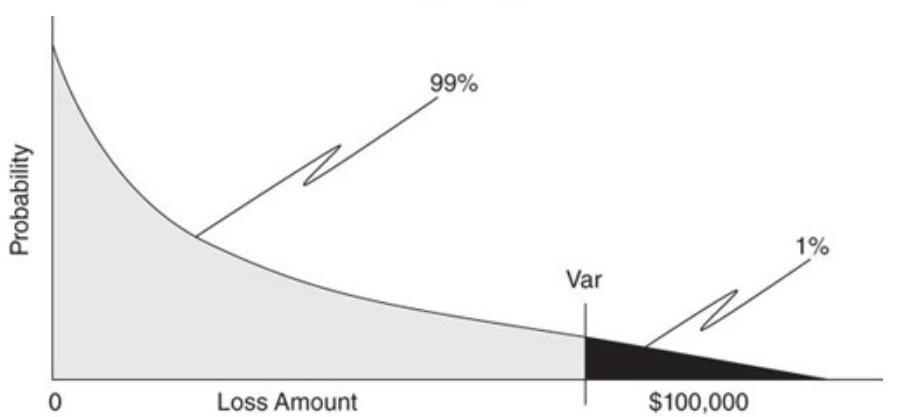
\includegraphics[max width=\textwidth]{2024_04_11_f382ae991e4e475fea0dg-4}
\end{center}

Example of the Distribution of a $\$ 100,000$ VaR for a Portfolio Based on a Confidence Level of $99 \%$

The VaR summarizes potential loss in a condensed and easy-to-understand way to facilitate understanding and comparison. However, as a single measure of potential loss, the information that it can contain is limited unless the user knows the shape of the distribution of the potential losses.

Variations of VaR exist, such as conditional value-at-risk. Conditional value-at-risk (CVaR), also known as expected tail loss, is the expected loss of the investor given that the VaR has been equaled or exceeded. Thus, if the VaR is $\$ 1$ million, then the CVaR would be the expected value of all losses equal to or greater than $\$ 1$ million. The CVaR provides the investor with information about the potential magnitude of losses beyond the VaR.

\section*{Strengths and Weaknesses of VaR}
The VaR provides a first glance at risk. It can be computed for a single risk exposure (such as a single security), for a portfolio, for an entire division, or for the entire firm. The VaR is a simplified risk measure that can be relatively uniformly computed and interpreted across divisions within a fund or across funds. Numerous entities request or require the reporting of VaR, and they test through time whether a fund's reported VaR is consistent with the actual risk that is experienced. The VaR is especially useful in situations in which a worst-case analysis makes no sense, such as in derivatives, where some positions have unlimited downside risk.

As a single risk measure, VaR provides rather limited information. Further, in some circumstances, VaR can be extremely deceptive. For example, consider a situation in which there is a 1 in 60 chance that a fund will lose $\$ 1$ million, and under all other situations, the fund will make $\$ 30,000$ (such as a fund writing an out-of-themoney binary option with a probability of being exercised of $1 / 60$ ). The VaR using $90 \%, 95 \%$, or $98 \%$ confidence is $\$ 0$. But the VaR using $99 \%$ confidence is $\$ 1$ million. A manager seeing only the $99 \%$ confidence number will perceive a very different risk exposure than a manager seeing VaR from a lower probability.

The VaR is an important risk measure and can be estimated in a variety of ways based on a variety of circumstances. The estimation of VaR is sufficiently important to warrant an entire section.


\end{document}